\RequirePackage[l2tabu,orthodox]{nag}

% TODO: decide if one-sided/two-sided
%\documentclass[headsepline,footsepline,footinclude=false,fontsize=11pt,paper=a4,listof=totoc,bibliography=totoc,BCOR=12mm,DIV=12]{scrbook} % two-sided % original source stated: BCOR=12mm,DIV=12
\documentclass[headsepline,footsepline,footinclude=false,oneside,fontsize=11pt,paper=a4,listof=totoc,bibliography=totoc,DIV=12]{scrbook} % one-sided

\usepackage{float}
\usepackage{graphicx}
\usepackage{placeins}
\usepackage{courier}
\usepackage{tikz}
\usepackage{caption}

\captionsetup{format=plain, font=small, labelfont=bf}
\usetikzlibrary{automata, positioning, arrows}

\tikzset{
        ->,  % makes the edges directed
        % >='stealth', % makes the arrow heads bold
        node distance=3cm, % specifies the minimum distance between two nodes. Change if n
        every state/.style={thick, fill=gray!10}, % sets the properties for each ’state’ n
        initial text=$ $, % sets the text that appears on the start arrow
        }

% TODO: change citation style in settings
\PassOptionsToPackage{table,svgnames,dvipsnames}{xcolor}

\usepackage[utf8]{inputenc}
\usepackage[T1]{fontenc}
\usepackage[sc]{mathpazo}
\usepackage[ngerman,english]{babel} % english is the same as american or USenglish
\usepackage[autostyle]{csquotes}
\usepackage[%
  backend=biber,
  url=true,
  style=numeric, % alphabetic, numeric
  sorting=none, % default == nty, https://tex.stackexchange.com/questions/51434/biblatex-citation-order
  maxnames=4,
  minnames=3,
  maxbibnames=99,
  giveninits,
  uniquename=init]{biblatex} % TODO: adapt citation style
\usepackage{graphicx}
\usepackage{scrhack} % necessary for listings package
\usepackage{listings}
\usepackage{lstautogobble}
\usepackage{tikz}
\usepackage{pgfplots}
\usepackage{pgfplotstable}
\usepackage{booktabs} % for better looking table creations, but bad with vertical lines by design (package creator despises vertical lines)
\usepackage[final]{microtype}
\usepackage{caption}
\usepackage[hidelinks]{hyperref} % hidelinks removes colored boxes around references and links
\usepackage{ifthen} % for comparison of the current language and changing of the thesis layout
\usepackage{pdftexcmds} % string compare to work with all engines
\usepackage{paralist} % for condensed enumerations or lists
\usepackage{subfig} % for having figures side by side
\usepackage{siunitx} % for physical accurate units and other numerical presentations
\usepackage{multirow} % makes it possible to have bigger cells over multiple rows in a table
\usepackage{array} % different options for table cell orientation
\usepackage{makecell} % allows nice manual configuration of cells with linebreaks in \thead and \makecell with alignments
\usepackage{pdfpages} % for including multiple pages of pdfs
\usepackage{adjustbox} % can center content wider than the \textwidth
\usepackage{tablefootnote} % for footnotes in tables as \tablefootnote
\usepackage{threeparttable} % another way to add footnotes as \tablenotes with \item [x] <your footnote> after setting \tnote{x} 


% https://tex.stackexchange.com/questions/42619/x-mark-to-match-checkmark
\usepackage{amssymb}% http://ctan.org/pkg/amssymb
\usepackage{pifont}% http://ctan.org/pkg/pifont
\newcommand{\cmark}{\ding{51}}%
\newcommand{\xmark}{\ding{55}}%


\usepackage[acronym,xindy,toc]{glossaries} % TODO: include "acronym" if glossary and acronym should be separated
\makeglossaries
\loadglsentries{pages/glossary.tex} % important update for glossaries, before document


\bibliography{bibliography}

\setkomafont{disposition}{\normalfont\bfseries} % use serif font for headings
\linespread{1.05} % adjust line spread for mathpazo font

% Add table of contents to PDF bookmarks
\BeforeTOCHead[toc]{{\cleardoublepage\pdfbookmark[0]{\contentsname}{toc}}}

% Define TUM corporate design colors
% Taken from http://portal.mytum.de/corporatedesign/index_print/vorlagen/index_farben
\definecolor{TUMBlue}{HTML}{0065BD}
\definecolor{TUMSecondaryBlue}{HTML}{005293}
\definecolor{TUMSecondaryBlue2}{HTML}{003359}
\definecolor{TUMBlack}{HTML}{000000}
\definecolor{TUMWhite}{HTML}{FFFFFF}
\definecolor{TUMDarkGray}{HTML}{333333}
\definecolor{TUMGray}{HTML}{808080}
\definecolor{TUMLightGray}{HTML}{CCCCC6}
\definecolor{TUMAccentGray}{HTML}{DAD7CB}
\definecolor{TUMAccentOrange}{HTML}{E37222}
\definecolor{TUMAccentGreen}{HTML}{A2AD00}
\definecolor{TUMAccentLightBlue}{HTML}{98C6EA}
\definecolor{TUMAccentBlue}{HTML}{64A0C8}

% Settings for pgfplots
\pgfplotsset{compat=newest}
\pgfplotsset{
  % For available color names, see http://www.latextemplates.com/svgnames-colors
  cycle list={TUMBlue\\TUMAccentOrange\\TUMAccentGreen\\TUMSecondaryBlue2\\TUMDarkGray\\},
}

% Settings for lstlistings

% Use this for basic highlighting
\lstset{%
  basicstyle=\ttfamily,
  columns=fullflexible,
  autogobble,
  keywordstyle=\bfseries\color{TUMBlue},
  stringstyle=\color{TUMAccentGreen}
}

% use this for C# highlighting
% %\setmonofont{Consolas} %to be used with XeLaTeX or LuaLaTeX
% \definecolor{bluekeywords}{rgb}{0,0,1}
% \definecolor{greencomments}{rgb}{0,0.5,0}
% \definecolor{redstrings}{rgb}{0.64,0.08,0.08}
% \definecolor{xmlcomments}{rgb}{0.5,0.5,0.5}
% \definecolor{types}{rgb}{0.17,0.57,0.68}

% \lstset{language=[Sharp]C,
% captionpos=b,
% %numbers=left, % numbering
% %numberstyle=\tiny, % small row numbers
% frame=lines, % above and underneath of listings is a line
% showspaces=false,
% showtabs=false,
% breaklines=true,
% showstringspaces=false,
% breakatwhitespace=true,
% escapeinside={(*@}{@*)},
% commentstyle=\color{greencomments},
% morekeywords={partial, var, value, get, set},
% keywordstyle=\color{bluekeywords},
% stringstyle=\color{redstrings},
% basicstyle=\ttfamily\small,
% }

% Settings for search order of pictures
\graphicspath{
    {logos/}
    {figures/}
}

% Set up hyphenation rules for the language package when mistakes happen
\babelhyphenation[english]{
an-oth-er
ex-am-ple
}

% Decide between
%\newcommand{\todo}[1]{\textbf{\textsc{\textcolor{TUMAccentOrange}{(TODO: #1)}}}} % for one paragraph, otherwise error!
%\newcommand{\done}[1]{\textit{\textsc{\textcolor{TUMAccentBlue}{(Done: #1)}}}} % for one paragraph, otherwise error!
% and
\newcommand{\todo}[1]{{\bfseries{\scshape{\color{TUMAccentOrange}[(TODO: #1)]}}}} % for multiple paragraphs
\newcommand{\done}[1]{{\itshape{\scshape{\color{TUMAccentBlue}[(Done: #1)]}}}} % for multiple paragraphs
% for error handling of intended behavior in your latex documents.

\newcommand{\tabitem}{~~\llap{\textbullet}~~}

\newcolumntype{P}[1]{>{\centering\arraybackslash}p{#1}} % for horizontal alignment with limited column width
\newcolumntype{M}[1]{>{\centering\arraybackslash}m{#1}} % for horizontal and vertical alignment with limited column width
\newcolumntype{L}[1]{>{\raggedright\arraybackslash}m{#1}} % for vertical alignment left with limited column width
\newcolumntype{R}[1]{>{\raggedleft\arraybackslash}m{#1}} % for vertical alignment right with limited column width

% TODO: change thesis information
\newcommand*{\getUniversity}{Technische Universität München}
\newcommand*{\getFaculty}{Department of Informatics}
\newcommand*{\getTitle}{Large Language Models as User Interfaces: Alignment In Well-Defined Problem Spaces}
\newcommand*{\getTitleGer}{Große Sprachmodelle als Benutzerschnittstellen: Abgleich in wohldefinierten Problemen}
\newcommand*{\getAuthor}{Andrei Bratu}
\newcommand*{\getDoctype}{Master's Thesis in Informatics}
\newcommand*{\getSupervisor}{Georg Groh}
\newcommand*{\getAdvisor}{Tobias Eder}
\newcommand*{\getSubmissionDate}{Submission date}
\newcommand*{\getSubmissionLocation}{Munich}


\newcommand{\pskip}{\vskip 0.2in}

\begin{document}

% TODO: decide on used language
%\selectlanguage{ngerman}
\selectlanguage{english}

% Set page numbering to avoid "destination with the same identifier has been already used" warning for cover page.
% (see https://en.wikibooks.org/wiki/LaTeX/Hyperlinks#Problems_with_Links_and_Pages).
\pagenumbering{alph}
\begin{titlepage}
  % HACK for two-sided documents: ignore binding correction for cover page.
  % Adapted from Markus Kohm's KOMA-Script titlepage=firstiscover handling.
  % See http://mirrors.ctan.org/macros/latex/contrib/koma-script/scrkernel-title.dtx,
  % \maketitle macro.
  \oddsidemargin=\evensidemargin\relax
  \textwidth=\dimexpr\paperwidth-2\evensidemargin-2in\relax
  \hsize=\textwidth\relax

  \centering

  \IfFileExists{logos/tum.pdf}{%
    \includegraphics[height=20mm]{logos/tum.pdf}
  }{%
    \vspace*{20mm}
  }

  \vspace{5mm}
  {\huge\MakeUppercase{\getFaculty{}}}\\

  \vspace{5mm}
  {\large\MakeUppercase{\getUniversity{}}}\\

  \vspace{20mm}
  {\Large \getDoctype{}}

  \vspace{15mm}
  \makeatletter
  \ifthenelse{\pdf@strcmp{\languagename}{english}=0}
  {\huge\bfseries \getTitle{}}
  {\huge\bfseries \getTitleGer{}}
  \makeatother

  \vspace{15mm}
  {\LARGE \getAuthor{}}

  \IfFileExists{logos/faculty.png}{%
    \vfill{}
    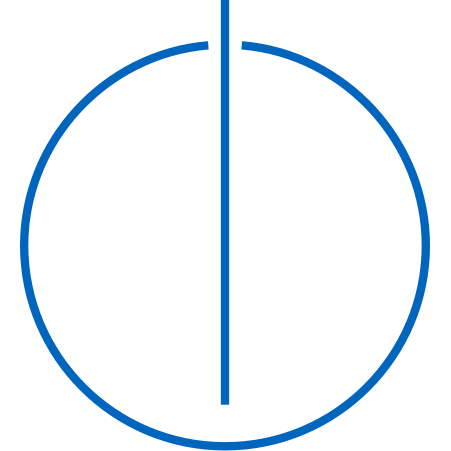
\includegraphics[height=20mm]{logos/faculty.png}
  }{}
\end{titlepage}


\frontmatter{}

\begin{titlepage}
  \centering

  \IfFileExists{logos/tum.pdf}{%
    \includegraphics[height=20mm]{logos/tum.pdf}
  }{%
    \vspace*{20mm}
  }

  \vspace{5mm}
  {\huge\MakeUppercase{\getFaculty{}}}\\

  \vspace{5mm}
  {\large\MakeUppercase{\getUniversity{}}}\\

  \vspace{20mm}
  {\Large \getDoctype{}}

  \makeatletter
  \vspace{15mm}
  \ifthenelse{\pdf@strcmp{\languagename}{english}=0}
  {
  {\huge\bfseries \getTitle{}}

  \vspace{10mm}
  {\huge\bfseries \foreignlanguage{ngerman}{\getTitleGer{}}}
  }
  {
  {\huge\bfseries \getTitleGer{}}

  \vspace{10mm}
  {\huge\bfseries \foreignlanguage{english}{\getTitle{}}}
  }
  \makeatother

  \vspace{15mm}
  \begin{tabular}{l l}
    Author:          & \getAuthor{} \\
    Supervisor:      & \getSupervisor{} \\
    Advisor:         & \getAdvisor{} \\
    Submission Date: & \getSubmissionDate{} \\
  \end{tabular}

  \IfFileExists{logos/faculty.png}{%
    \vfill{}
    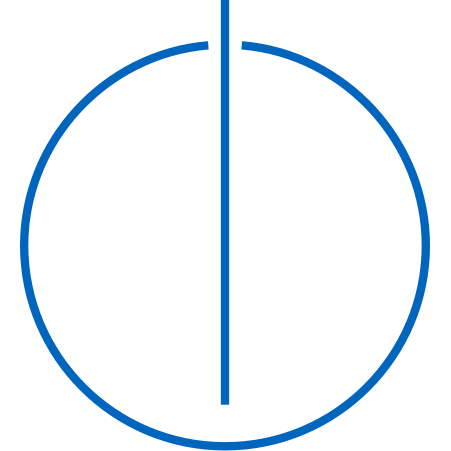
\includegraphics[height=20mm]{logos/faculty.png}
  }{}
\end{titlepage}

\cleardoublepage{}

\thispagestyle{empty}
\vspace*{0.8\textheight}
\noindent
\makeatletter
\ifthenelse{\pdf@strcmp{\languagename}{english}=0}
{I confirm that this \MakeLowercase{\getDoctype{}} is my own work and I have documented all sources and material used.}
{Ich versichere, dass ich diese \getDoctype{} selbstständig verfasst und nur die angegebenen Quellen und Hilfsmittel verwendet habe.}
\makeatother

\vspace{15mm}
\noindent
\getSubmissionLocation{}, \getSubmissionDate{} \hspace{50mm} \getAuthor{}

\cleardoublepage{}

\newpage


\vspace*{\fill}
\centering
All models are approximations. Essentially, all models are wrong, but some are useful. However, the approximate nature of the model must always be borne in mind.

\centering\textbf{George Edward Pelham Box FRS, British Statistician}
\vspace*{\fill}
\makeatletter
\ifthenelse{\pdf@strcmp{\languagename}{english}=0}
{\addcontentsline{toc}{chapter}{Acknowledgments}}
{\addcontentsline{toc}{chapter}{Danksagungen}}
\makeatother
\thispagestyle{empty}

\vspace*{20mm}

\begin{center}
\makeatletter
\ifthenelse{\pdf@strcmp{\languagename}{english}=0}
{\usekomafont{section} Acknowledgments}
{\usekomafont{section} Danksagungen}
\makeatother
\end{center}

\vspace{10mm}

This work has been carried out under the patronage of the prestigious industry partner Bayerische Motoren Werke AG, and the collegiate of the creative ZI-222 research department. Computing power and technical sophistication must always translate in a better, easier or at least more entertaining life for humans. Our shared vision of using natural language to command the intelligent devices we surround ourselves with, including automotive vehicles, has resulted in this labour of love.

I would like to offer thanks to Lukas Stappen and Tobias Eder for their guidance and never-ending patience.

\cleardoublepage{}
 % TODO: if you don't have anyone to thank for or don't wish to publish it, comment this line out.
\chapter{\abstractname}

Large language models represent a milestone in the discipline of natural language processing. Their ability to adapt to novel tasks without further training, using few to no demonstrations, matches the definition of intelligence as the ability to solve complex problems and achieve goals. A sizeable portion of the literature investigates the presence of 'common sense', 'reasoning' or 'problem-solving' in such models.
 
This work investigates the use of large language models as user interfaces: mediators between humans and computing systems. The model interprets a query presented in natural language and then delegates work to sub-modules, or tools, that impact the system's state. Such problems are deemed in the scope of this work as "well-defined": the desired changes to the system's state are either present or inferrable from the query, and there is a clear mapping between properties of the system and the tool or chain of tools required to modify it, and the properties of the state tend to be themselves finite or in defined ranges. Such well-defined problems are contrasted by the more abstract and creative tasks such as creating writing materials, writing program code snippets or knowledge queries.

The investigation introduces the "oracle hypothesis": large language models have an innate understanding of human expectations and can anticipate the desired end state from the query. They are, however, incapable of forming a plan of action to achieve the desired end state. The prompting and reasoning strategies found in the literature are ineffective due to a bias of datasets representative of the second problem class. Leveraging the well-defined nature of the controller scenario, novel prompting and fine-tuning techniques are developed for user-model alignment. 



\makeatletter
\ifthenelse{\pdf@strcmp{\languagename}{english}=0}
{\renewcommand{\abstractname}{Kurzfassung}}
{\renewcommand{\abstractname}{Abstract}}
\makeatother

\chapter{\abstractname}

%TODO: Abstract in other language
\begin{otherlanguage}{ngerman} % TODO: select other language, either ngerman or english !

\end{otherlanguage}


% Undo the name switch
\makeatletter
\ifthenelse{\pdf@strcmp{\languagename}{english}=0}
{\renewcommand{\abstractname}{Abstract}}
{\renewcommand{\abstractname}{Kurzfassung}}
\makeatother
\microtypesetup{protrusion=false}
\tableofcontents{}
\microtypesetup{protrusion=true}

\mainmatter{}

\newtheorem{definition}{Definition}

% !TeX root = ../main.tex
% Add the above to each chapter to make compiling the PDF easier for some editors.

\chapter{Introduction}\label{chapter:introduction}

% \section{Section}
% Citation test (with Biber)~\parencite{latex}.

\section{Paradigm Shift}

The Transformer architecture is pervasive in modern natural language processing. First introduced by Vaswani et al. \cite{DBLP:journals/corr/VaswaniSPUJGKP17}, it was originally applied to the sequence-to-sequence problem in language translation. The mapping from $X \in \mathbb{R}^{n \times d}$ to $Y \in \mathbb{R}^{n \times d}$ is complex, as the mapping of each individual element $x_i$ in the sequence must account for the entire context window $X$.

\vskip 0.2in

This problem arises in natural language processing, where mapping between sequence domains is common in tasks like machine translation (mapping between two different languages) or text summarization (mapping from an ‘expanded’ version to a more ‘condensed’ one within the same language). The concept has also been extended to other fields, such as image understanding, and has enabled cross-domain applications like text-to-image or image-to-text generation, demonstrating the versatility and universal applicability of the architecture.

\vskip 0.2in

To address the challenge of context-dependent, cross-domain mapping, Transformers utilize multiple \textbf{attention blocks} designed to learn context-aware mappings. Three projection matrices, $W^Q$, $W^K$, and $W^V$, are learned. When multiplied with the input $X$, they yield $Q$, $K$, and $V$, respectively. These tensors function as a differentiable lookup table: the key vector $k_i$ is multiplied by the query vectors $q_i$ at all positions to determine the relevance of other positions for position $i$. The $V$ matrix then uses the attention scores to compute the final embedding $Z$ of $X$.

\begin{figure}[h]
\[ Z = softmax(\frac{QK^T}{\sqrt{d_k}})VW^O \text{, where } Q = XW^Q\text{, }K = XW^K\text{, } V = XW^V \]
\caption[Attention Equation]{The attention equation. The softmax function is used to map attention scores at each position to a probability distribution. Scaling by the size of the key vectors, $d_k$, is applied to normalize these values. A final linear layer, $W^O$, is applied to the computed attention vectors, resulting in the final latent representation.}
\end{figure}

\vskip 0.2in

Transformers divide their architecture into two main components: the encoder and the decoder. Each section consists of multiple stacked attention layers to create more powerful mappings. However, the authors introduce two key modifications in the decoder. First, the encoder’s output is treated as a universal latent representation of the input, so the decoder layers project $W^Q$ onto the final encoder output, $Z^{e}$, instead of using the decoder’s input vectors. Second, since the decoder generates sequences one step at a time, using the context $\overline{i+1..n}$ to compute the current position $i$ would be incorrect. To address this, future positions are masked during training. Finally, the output of the last attention layer in the decoder is passed through a classification head to generate the desired sequence $Y$.

\begin{figure}[h]
\[ Z^d = softmax(\frac{QK^T + M}{\sqrt{d_k}})VW^O \text{, where } Q = Z^eW^Q\text{, }K = XW^K\text{, } V = XW^V \]
\caption[Decoder Modification in Transformer Architecture]{The three linear layers in attention reformulated with decoder constraints. Here, $X$ represents the output of the previous attention layer in the decoder. $M$ is a mask applied over the attention filter to block future values by adding a “negative infinity” value below the second diagonal. This modification is referred to as cross-attention in the literature, distinguishing it from the encoder’s ‘self-attention’ mechanism.}
\end{figure}

At their core, Transformers build upon several foundational concepts in deep learning. Convolutional neural networks (CNNs) create context-aware representations using a smaller sliding window to downscale high-dimensional vectors, particularly in image processing. Recurrent neural networks (RNNs) similarly aim to capture context-aware embeddings by computing position $i$’s embedding based on state embeddings that encode previous positions (or, in some variants, both past and future windows). Earlier architectures, like U-NET by Ronneberger et al. \cite{ronneberger2015unetconvolutionalnetworksbiomedical}, also employed latent representations to map from one domain to another. However, Transformers surpass these models by utilizing the full context of the sequence at all times and introducing a simplified architecture that enables highly parallel computation, unlike the sequential backpropagation through time used in RNNs.

\pskip

From the perspective of an \gls{nlp} practitioner at the start of this decade, Transformers represented an incremental improvement in the deep learning paradigm, rather than a revolutionary shift. Yet, this same architecture has since sparked debates about the potential for general artificial intelligence \cite{bubeck2023sparksartificialgeneralintelligence}. OpenAI’s \gls{gpt} family of language models builds on the Transformer architecture, specifically using its decoder to generate text continuations from word embeddings based on user input. Unlike traditional language models, \gls{gpt} models are trained on vast text corpora, with parameter counts several orders of magnitude larger. This difference in scale involves hundreds of gigabytes of training data, sourced from web crawls, and models with hundreds of billions of parameters.

\pskip

Beginning with the GPT-3 iteration, the model demonstrated emergent and unexpected behaviors. Unlike traditional models, which are typically trained for a single task using one or more closely related datasets, GPT-3 exhibited few-shot and even zero-shot capabilities. With zero or only a few examples provided in the prompt, the model could perform at a level comparable to state-of-the-art models on diverse, unrelated tasks, including question answering, basic arithmetic, reasoning, translation, and summarization.

\begin{figure}[h!]
    \centering
    \captionsetup{format=plain, font=small, labelfont=bf}
    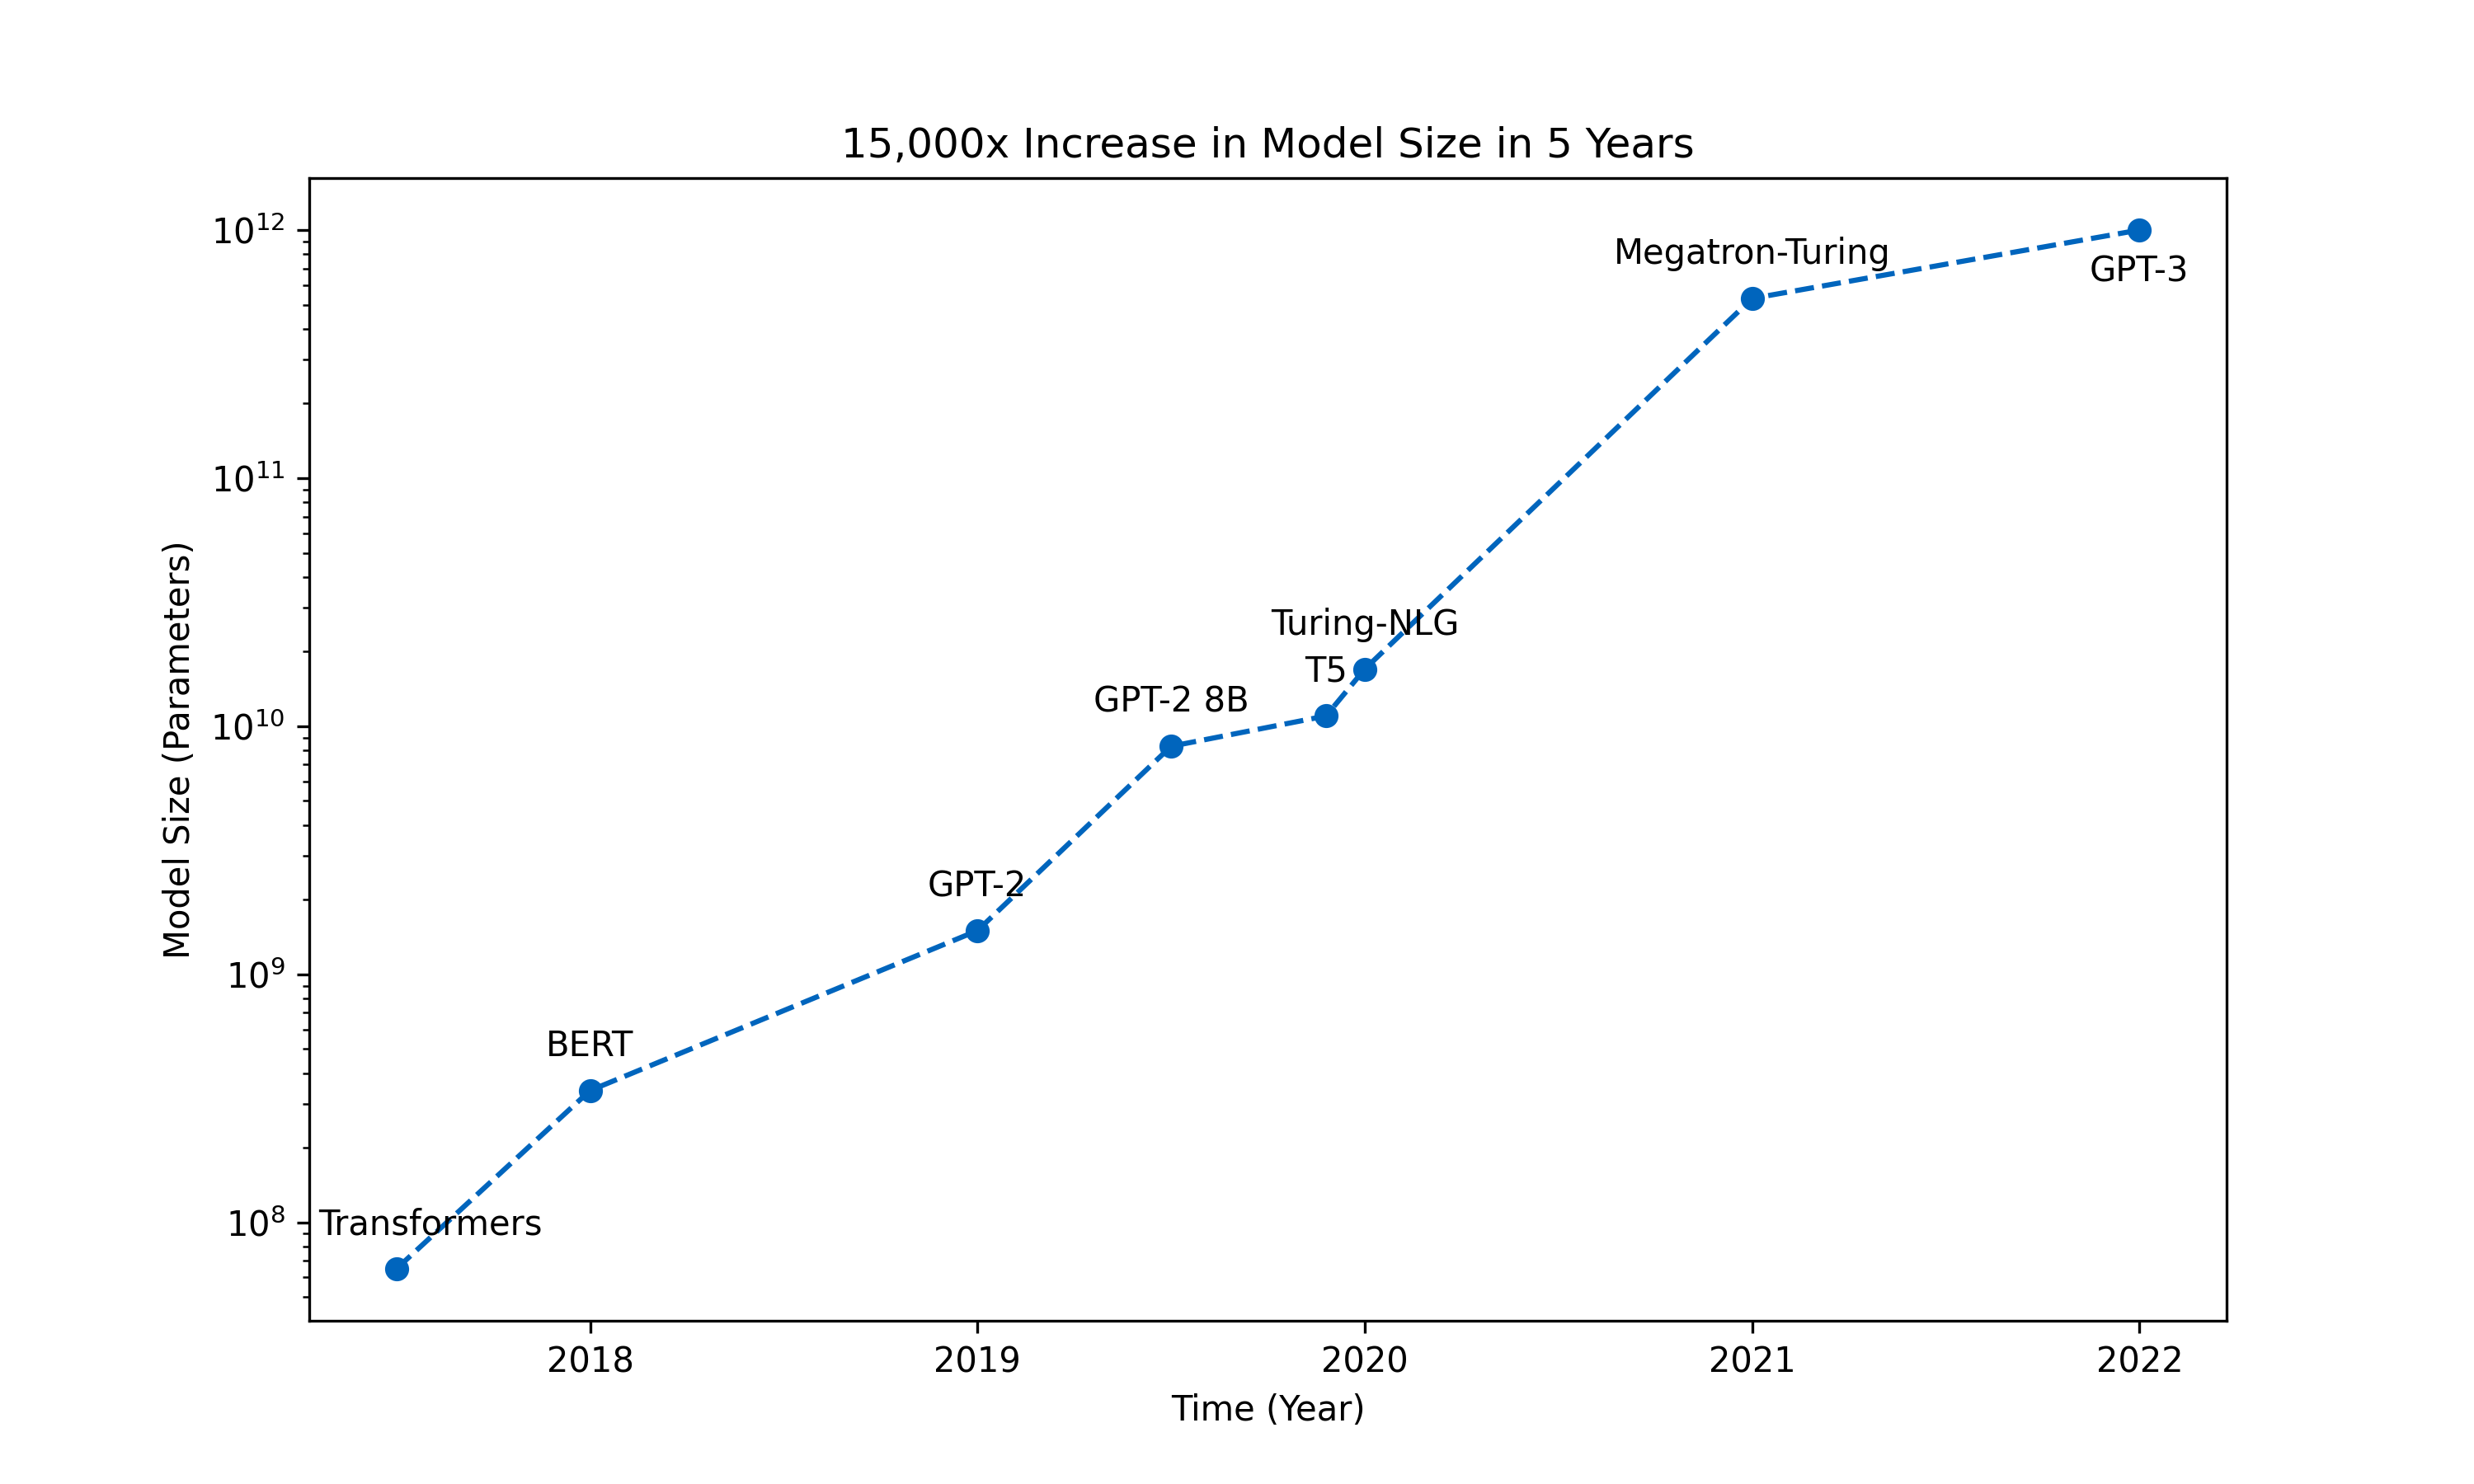
\includegraphics[width=\linewidth]{figures/modelsizeincrease.png}
    \caption[Progression of Models Size in \glspl{llm}]{The exponential increase in the number of parameters in \glspl{llm} is the main cause of their few-shot capabilities.}
    \label{fig:sample_plot}
\end{figure}

Such behavior has been previously observed to some extent within the field of meta-learning. Meta-learning aims to create meta-objectives for optimization, such as using meta-models trained on related but distinct tasks—like training the same machine translation model on multiple language pairs to enhance generalization with fewer examples. Some approaches explore meta-objectives by introducing penalties for using large training datasets, encouraging the discovery of parameter configurations that can be fine-tuned with minimal data on new tasks. Additionally, meta-optimizers are studied to fine-tune optimizers for more efficient training across families of functions \cite{metalearning}.

\pskip

While these methods have led to improved generalization, they also introduce complex training procedures involving second-order optimizations. Moreover, they require significant expert involvement \cite{Yao2018TakingHO}, and some argue that they merely shift the problem of distribution mismatch \cite{wiles2021finegrainedanalysisdistributionshift}, as models can still be applied to data distributions that differ from those seen during training.

\pskip

Given the challenges and extensive human effort invested in improving individual models, the prospect of training a single model and applying it across all tasks naturally garnered the attention of the scientific community. This has led to large language models (LLMs) being referred to as \glspl{fm} (foundational models) \cite{foundationalmodels}. The power and versatility of these models have also attracted interest from fields such as psychology and human-computer interaction. Surveys analyzing social media posts reveal public curiosity about these models, with users testing complex, human-like behaviors such as humor and irony while exploring the models’ capabilities \cite{Dynel2023}.

\pskip

In writing tasks, LLMs are increasingly used in both academic and practical contexts, such as emails or letters. Users’ ‘cognitive appreciation’—the recognition of the model’s utility—often surpasses their initial ‘emotional appreciation’ for its human-like interactions. However, while users tend to view these models positively as assistants, they remain cautious about the accuracy of the information provided \cite{Luther2024} \cite{XinXiaCao2023} \cite{Herbold2023}.

\pskip

Human intelligence is often defined by the ability to learn and apply previously acquired knowledge to new tasks \cite{Sternberg2012}. By this definition, \glspl{llm} could be considered intelligent, as they can process new information and accomplish goals. However, the nature of this intelligence differs fundamentally from human intelligence. \glspl{llm} are stochastic models that predict and output the next most likely word based on the given context, similar in principle to \gls{ngram} models \cite{brown1992class}.

\section{Prompting Intelligence}

Having contextualized the rise of \glspl{llm} and the paradigm they have established, it is essential to discuss how the capabilities of \glspl{fm} are being utilized. While their usefulness in downstream writing tasks is evident, the research community has naturally sought to systematize methods for evaluating \glspl{fm}. This section provides an overview of how end users adapt queries presented to \glspl{llm} to achieve specific goals and examines how \gls{nlp} practitioners measure intelligence.

\pskip

In the context of \glspl{llm}, the input provided by the user is referred to as a \textbf{prompt}, which is crafted to instruct the model on the desired task. The literature differentiates between two prompting techniques: zero-shot and few-shot prompting.

\pskip

Zero-shot techniques guide the model’s text output by instructing it to adopt a specific communication style, express a particular emotion \cite{emotionalstimuli} \cite{boundingcapacities}, or roleplay as a specific individual, such as a personal assistant or a domain expert \cite{roleplaying} \cite{helpfulassistant}. In contrast, few-shot techniques \cite{gpt3} include examples, called \textbf{demonstrations}, within the prompt to illustrate the expected output for the task. Research shows that prompts resembling formats commonly seen in training data \cite{Jiang2020}, including demonstrations, using diverse demonstrations that cover a broader range of labels \cite{su2022selectiveannotationmakeslanguage} \cite{min2020ambigqaansweringambiguousopendomain}, and customizing the demonstration format (e.g., not relying solely on a fixed format like \verb+{“Q:  A: ”}+) \cite{Jiang2020} all improve task performance.

\pskip

However, some research suggests that even minor, seemingly irrelevant changes to prompts can affect model behavior, and that the correctness of labels in demonstrations is less crucial than ensuring broad representation of possible labels \cite{min2020ambigqaansweringambiguousopendomain} \cite{wei2023chainofthoughtpromptingelicitsreasoning}. This is particularly important given the potential limitations of the model’s context window. These findings highlight the constraints of foundational models, previously perceived as all-encompassing. In response, methods like prompt mining \cite{Jiang2020} and K-Nearest Neighbors for selecting demonstrations that more closely resemble the test dataset \cite{liu2021makesgoodincontextexamples} have been developed to address these limitations.

\begin{figure}[H]
\centering
\fbox{
\begin{minipage}{39em}

\captionsetup{format=plain, font=small, labelfont=bf}

\textbf{Task: Explain a historical event while assuming the persona of a real person.}

\vskip 0.2in

\textbf{Prompt}: Explain what happened at Roswell as if you were Youtuber Michael from  Vsauce.

\vskip 0.1in

\textbf{Model}: Hey, Vsauce, Michael here. But what really is here when you think about outer space? That brings us to Roswell, New Mexico, and the most famous alleged UFO incident in history...

\rule[1ex]{.2\textwidth}{.5pt}

\textbf{Prompt}: Explain what happened at Roswell as if you were Donald Trump.

\vskip 0.1in

\textbf{Model}: Let me tell you about Roswell, folks. Many people are talking about it—big mystery, very interesting! Back in 1947, something incredible happened in Roswell, New Mexico. This wasn’t just any balloon...

\rule[1ex]{\textwidth}{1pt}

\textbf{Task: Writing an email message that takes user's relationship with the addressed into consideration.}

\vskip 0.2in

\textbf{Prompt}: Tell my boss I am going to take two days off. We are not on good terms so emphasize I need them for health concerns.

\textbf{Model}: 
Subject: Request for Sick Leave

Dear [Boss’s Name],

I hope this message finds you well. I am writing to inform you that I am currently experiencing some health concerns that require immediate and comprehensive attention...

\rule[1ex]{.2\textwidth}{.5pt}

\textbf{Prompt}: Tell me boss I am going to take two days off. We are buddies so keep it friendly and short.

\textbf{Model}: 
Hey [Boss’s Name],

Just a heads up, I need to take a couple of days off for some health stuff. Planning on being out [insert days]. I’ll make sure everything’s covered before I go...

\end{minipage}
}
\caption[Examples of zero-shot prompting techniques]{Examples of zero-shot prompting techniques. By altering the prompt, the users can control the output, highlighting the facile user experience that have made foundational models popular.}
\end{figure}

While these methods yield strong results in practical applications, they often rely on human feedback and subjective judgment to evaluate model performance. In contrast, researchers continue to apply \glspl{fm} to standardized \gls{nlp} task datasets, such as those for translation or summarization, to benchmark their capabilities. Additionally, there is growing interest in testing \glspl{llm} on tasks that assess more complex, intelligent behaviors, such as shared knowledge \cite{talmor2019commonsenseqaquestionansweringchallenge}, reading comprehension \cite{zhang2018recordbridginggaphuman}, and arithmetic \cite{cobbe2021trainingverifierssolvemath}.

\pskip

To enhance performance on these more demanding tasks, researchers have identified three main approaches. The most common is \gls{cot} (Chain of Thought), which prompts the model to provide not just an answer but also an explanation of its reasoning process \cite{wei2023chainofthoughtpromptingelicitsreasoning}. Variants of \gls{cot} include generating solutions step by step, with user feedback at each stage \cite{zhou2023threadthoughtunravelingchaotic}, prompting the model for high-level, relevant knowledge \cite{zheng2024stepbackevokingreasoning}, or applying \gls{cot} to training examples and sampling similar solved examples for testing \cite{li2024dialoguepromptingpolicygradientbaseddiscrete}. 

\pskip

The other two approaches include decomposing complex problems into simpler sub-questions and solving each individually \cite{patel2022questiondecompositionunitneed} \cite{wang2023planandsolvepromptingimprovingzeroshot}, or using multiple prompts and selecting the answer supported by a majority vote \cite{khalifa2023exploringdemonstrationensemblingincontext} \cite{wang2023selfconsistencyimproveschainthought}.

\pskip

 With an understanding of how intelligence is measured in \glspl{llm}, we can revisit the perspective on intelligence discussed in the previous section. According to the \Gls{act} framework of cognition \cite{Anderson2013}, intelligent behavior is rooted in three types of knowledge. Declarative knowledge encompasses the facts and goals an intelligent agent seeks to achieve, while procedural knowledge consists of production rules that generate new knowledge or behaviors based on the agent’s current 'working memory' chunks. Human agents blend these two forms of knowledge to navigate novel situations or reprioritize tasks.

 \pskip

Previous statistical models heavily relied on declarative knowledge, such as using context to generate the next word or applying training data to solve similar examples. In contrast, \glspl{llm} seem capable of drawing on internalized production rules to address novel, unseen problems. For instance, they can imitate the speech mannerisms of a specific person to generate coherent output on topics the person has never discussed.

\pskip

Critics, however, argue that this capability may be a form of overfitting. With vast numbers of parameters and access to large corpora, \glspl{llm} can allocate resources for a wide range of input scenarios. This critique mirrors concerns raised against DeepMind's reinforcement learning agents in Vinyals et al., where the AI agents’ extensive training, amounting to decades of human experience, allowed them to observe a far greater portion of game states. As a result, their superhuman performance was seen as philosophically inferior to human intelligence, which internalizes rules more quickly and applies them flexibly to new situations \cite{Vinyals2019}. Similarly, while the procedural knowledge exhibited by \glspl{fm} may be viewed as inferior to human capabilities, it is still present.

\section{Rise of Language Agents}

The previous sections have argued for the presence of intelligent behavior in \glspl{llm}, but their usage also introduces significant limitations and risks. One major concern is the high energy consumption required for training, which, when combined with uncurated data scraped from the internet, can reinforce harmful biases and discrimination in decision-making systems, such as those used for hiring \cite{parrots}. Additionally, since \glspl{llm} are trained on data up to a specific cutoff date, they lack awareness of information produced after that point and may perform poorly on topics with limited data, such as specialized fields. The phenomenon of generating factually incorrect or misleading outputs, commonly referred to as \textbf{hallucinations}, has also been well-documented \cite{bai2024hallucination}.

\pskip

To address these issues, ongoing research aims to mitigate harmful or undesirable outputs. One prominent approach is \gls{rlhf} (Reinforcement Learning with Human Feedback), where human users provide feedback on the quality of generated text, either through binary ratings or numerical scores. This feedback is used to train a neural network that serves as a reward function for the model or policy, in the language of \gls{rl}. The reward function then fine-tunes the policy to align the model with human values, such as promoting usefulness or avoiding harmful stereotypes \cite{ouyang2022traininglanguagemodelsfollow}.

\pskip

Another approach involves developing guardrails for \glspl{llm}’ outputs. These guardrails may include hard-coded rules, such as avoiding specific keywords, or use the model itself to critique its output based on predefined principles written in natural language \cite{dong2024buildingguardrailslargelanguage} \cite{yuan2024rigorllmresilientguardrailslarge}.

\pskip

The future trend in working with \glspl{llm} is shifting toward a more integrated approach in both academia and industry. As discussed, these models have exhibited behavior that increasingly aligns with our understanding of human intelligence. Their true potential lies in leveraging up-to-date knowledge bases while delegating specialized tasks to external tools, such as calculators or logical provers \cite{Trinh2024}. These tools can be easily integrated through text formats like \Gls{json}. When paired with a retrieval system, the rate of hallucinations in \glspl{llm} decreases significantly \cite{ding2024survey} \cite{wang2024evaluating}. 

\pskip

Given the intelligent behavior exhibited by \glspl{fm}, the trust they garner from users, and their ability to delegate specialized tasks, \glspl{fm} are poised to become the next widely adopted \Gls{ui}, much like the mouse and keyboard for personal computers or the touchscreen for handheld devices.

\begin{figure}[h!]
    \centering
    \captionsetup{format=plain, font=small, labelfont=bf}
    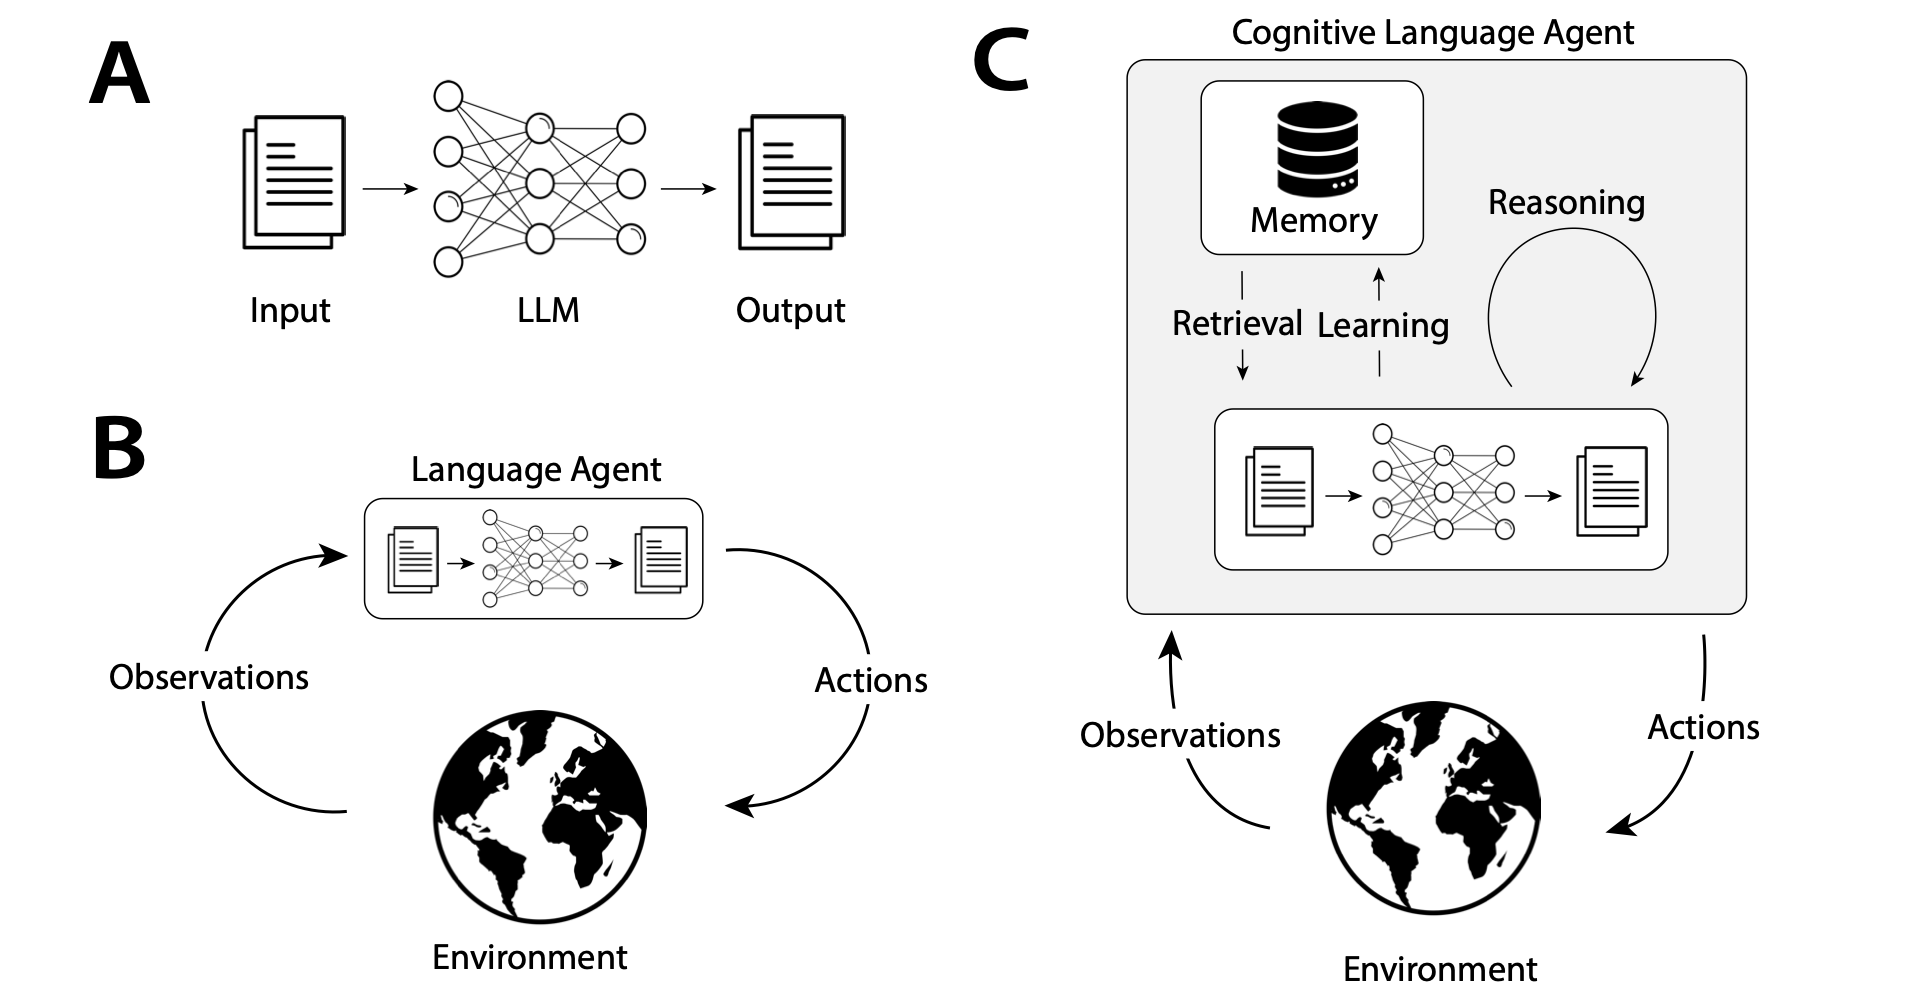
\includegraphics[width=\linewidth]{figures/cognitive_architectures.png}
    \caption[Illustration of Cognitive Architectures for Human Agents]{Reproduced from *Cognitive Architectures for Language Agents* by Sumers et al. \cite{sumers2024cognitivearchitectureslanguageagents}. The usage of \glspl{llm} is shifting towards human-aligned models (B) that interface with external tools to interact with an environment (C), rather than solely generating text as a response (A). The emergent abilities of large language models are increasingly being utilized to direct or delegate tasks to external systems, positioning them as intermediaries between computing systems and human users through the medium of natural language.}
    \label{fig:enter-label}
\end{figure}

\pskip

This idea has been echoed by Mei et al. \cite{aiasos}, who envision an operating system kernel responsible for system calls and process scheduling, paired with a language agent kernel that manages tasks such as context window management, information retrieval, and delegation to specialized language agents. In this framework, traditional programs expose a natural language interface, allowing programs to be controlled through natural language commands, with the \glspl{llm} kernel delegating user inputs accordingly.

\section{An Epistemiological Gap}

Our work has reviewed the current research on language agents to assess the state of the field. It reveals that the topic is still developing, with much of the research focused on traditional tasks like translation, mathematical reasoning, or general knowledge processing. Specifically, 83 papers on the topic of \glspl{llm} using tools were identified by counting the papers that cite *Cognitive Architectures for Language Agents* by Sumers et al. \cite{sumers2024cognitivearchitectureslanguageagents}. This is overshadowed by the broader body of research on \glspl{llm}, with 31,425 papers citing the ChatGPT-3 model's accompanying article \cite{gpt3}. Notably, the topic of \glspl{rag} (retrieval-augmented generation) intersects with various \glspl{llm} research areas, and the count of papers related to \glspl{llm} using tools has been refined to exclude those primarily focused on \glspl{rag}. Additionally, one prominent paper, *ToolLLM: Facilitating Large Language Models to Master 16000+ Real-world APIs* \cite{qin2023toolllmfacilitatinglargelanguage}, has 341 citations, suggesting an upper bound of around 400 papers on language agents.

\pskip

In *Gorilla: Large Language Model Connected with Massive APIs*, Patil et al. \cite{patil2023gorillalargelanguagemodel} fine-tune a ChatGPT-4 architecture to interact with 1,645 APIs. These APIs represent deep learning models hosted on repositories like TorchHub and Hugging Face, which can be accessed using standardized code methods. The model employs the Self-Instruct paradigm \cite{selfinstruct} to generate synthetic user query-API call examples based on documentation from these repositories. An Abstract Syntax Tree is used to verify valid code generations, which are then used to further fine-tune the architecture. The model is also integrated with a \gls{rag} system, which updates API documentation and retrieves the most relevant tools for the user's query. This allows the \gls{llm} to respond to diverse queries, from natural language translation to image manipulation. The authors have continued to develop this approach through an open-source project, *OpenFunctions-v2*, which supports arbitrary functions and allows for multiple or parallel function calls.

\pskip

In \textit{ToolLLM: Facilitating Large Language Models to Master 16000+ Real-world APIs}, Qin et al. \cite{qin2023toolllmfacilitatinglargelanguage} utilize an API repository that indexes numerous APIs and provides a unified interface for querying them. Similar to the approach by Patil et al., the authors fine-tune \glspl{llm} on synthetic demonstrations and employ a \gls{rag} system to adapt to new, unseen APIs as they are scraped and added to the repository. The process is further refined through a depth-first exploration strategy, which generates multiple execution plans for a user query and prunes them to identify the most promising one. Solutions are evaluated using two metrics: the \textbf{pass} metric, where a \gls{llm} evaluator judges whether the final answer aligns with the user's query intent, and the \textbf{win} metric, which compares the quality of one solution against another. It is worth noting that the APIs are not filtered, resulting in functional duplicates within the 16,000-strong tool environment leveraged by the agent.

\pskip

The review of language agent literature leads to several key conclusions. First, reasoning in language agents is heavily dependent on the \textbf{query intention}. Human assessment or relying on \glspl{llm} to evaluate human judgments \cite{zheng2023judgingllmasajudgemtbenchchatbot} is essential for benchmarking \glspl{llm} performance, differing from much of the \glspl{llm} literature that evaluates reasoning or common sense by comparing outputs to a predefined correct answer. Second, current research is focused on developing \textbf{universal language agents}, capable of integrating a wide range of tools and selecting the most relevant ones through a \gls{rag} system based on the user's query. However, this introduces latency, making it difficult to scale these systems for real-world applications. As noted by Mei et al. \cite{aiasos}, a more feasible implementation of \glspl{llm} as user interfaces is likely to involve complementing traditional user interfaces—whether physical or software-based—with a natural language interface that translates user queries into a predefined set of functionalities. Third, a scalable approach involves using \glspl{llm} to generate synthetic examples or evaluations, aligning the models with the ability to utilize tools effectively.

\pskip

This brief overview of language agents contrasts with the broader trends in \glspl{llm} research. Most \glspl{llm} are evaluated using a train-validation-test split, with their output compared against a gold standard answer. Methods like \gls{cot} (Chain of Thought) are designed for this workflow, leveraging the information in the prompt and the knowledge internalized by the \gls{llm} during training to generate responses. In contrast, language agents rely less on drawing out latent knowledge and more on their ability to interpret the user's intent and delegate tasks to external systems or functions.

\pskip

This work focuses on training language agents to serve as interfaces for computing systems. It seeks to bridge the gap between mainstream \gls{llm} research and the specialized subfield of language agents, questioning whether existing prompting methods can enhance performance in this context or if new techniques must be developed. The work is rooted in practical application. While current research on language agents is primarily concerned with building universal agents capable of interfacing with a wide range of tools, this work assumes that industry professionals may favor a different approach. In scenarios where low latency and precision in interpreting user queries are crucial, it is expected that specialized models, fine-tuned for known toolsets, will be preferred—especially when \gls{rag} systems are unavailable and accurately modeling user intent is critical.

\pskip

An important assumption in this work is that the systems with which language agents interface—whether physical or software—have a well-defined purpose. The state of the system is defined by a finite number of attributes, each with values from a finite domain. The user interacts with the system by transitioning it from one state to another. In this context, the language agent's role is to move the system from its current state to the user's desired state, determining the optimal path using available tools, which can be conceptualized as a state machine. This focus is reflected in the subtitle, \textbf{Alignment in Well-Defined Problem Spaces}, and will be explored in depth in the second chapter, where the problem is formally defined. These assumptions enable the exploration of language agents as user interfaces through the following research questions:

\pskip

\textbf{Q1: Are language models capable of understanding user intent? Can we quantify this understanding?}

\vskip 0.1in

As demonstrated by Zheng et al. \cite{zheng2023judgingllmasajudgemtbenchchatbot}, \glspl{llm} are competent approximators of human intent, and they are often used to assess the quality of output generated by other \glspl{llm} in language agents \cite{qin2023toolllmfacilitatinglargelanguage}. By modeling controlled cyber-physical systems as state machines with known attributes, we can numerically quantify how well \glspl{llm} anticipate the user's desired end state. This is achieved by comparing the model-predicted end state with expert human opinion and the actual end state reached through the model’s execution plan. This comparison provides valuable insights into improving language agents. For the scope of this work, we refer to this measure as *alignment*, which is rooted in the \textit{oracle hypothesis} presented in the following chapter.

\pskip

\textbf{Q2: Can language agents handle complex queries with multiple objectives or dependencies?}

\vskip 0.1in

As noted, current research on language agents primarily focuses on equipping \glspl{llm} with numerous tools, transforming them into universal agents. In contrast, this work aims to push the boundaries by testing language agents' ability to manage more complex scenarios involving multiple parallel objectives, conditional execution flows, and tool dependencies. To facilitate this, a novel dataset is proposed, emphasizing these challenges. A comparison between this dataset and existing datasets in the language agent literature will be presented in Chapter \ref{chapter:problem_definition}, \textbf{Problem Definition}.

\pskip

\textbf{Q3: How efficient are current prompting strategies for language agents?}

\vskip 0.1in

In line with the constraints of well-defined systems, the language agents in this study will be prompted to generate structured action plans to fulfill the user’s query with minimal latency. Most existing prompting strategies are developed and evaluated under a different framework than that of language agents, raising concerns about an "epistemological gap." We evaluate various prompting strategies based on the alignment metric from \textbf{Q1} and the executability of the generated plans—that is, whether the plan generated by the language agent can be executed and is logically sound. Additionally, we investigate whether the \gls{json} format is optimal for queries in our dataset, given the output's reliance on task prompt quality, as discussed in Section \ref{chapter:prompting_techniques}.

\pskip

\textbf{Q4: Are there fine-tuning methods that improve language agent performance on our defined problem?}

\vskip 0.1in

By conceptualizing the interaction between language agents and systems as state machines, the execution of one or more tools can be mapped to system state transitions. Given that \glspl{llm} are proficient at approximating human intent \cite{zheng2023judgingllmasajudgemtbenchchatbot}, we hypothesize that language agents struggle to fully "understand" how tool usage impacts the system's state. This work explores this hypothesis and develops a novel fine-tuning technique based on this insight. The approach is compared to a naive method, where the model is simply presented with a query and its corresponding plan.

\pskip

In the following chapters, we address the research questions and methodologies of this study, exploring well-defined systems, experimental design, and performance evaluation of language agents interfacing with cyber-physical systems.

\pskip

Chapter two formalizes well-defined systems, outlines the study's constraints, and introduces the simulated system and a novel benchmarking dataset, comparing it with two existing datasets.

\pskip

Chapter three details the experimental setup, evaluates various prompting strategies, identifies sources of errors in \glspl{llm}' execution plans, and compares the \gls{json} and \gls{gml} formats for plan representation.

\pskip

Chapter four presents a fine-tuning technique based on system state transitions and compares its performance with both a baseline and naive fine-tuning method across all strategies.



% !TeX root = ../main.tex
% Add the above to each chapter to make compiling the PDF easier in some editors.


\chapter{Problem Definition}\label{chapter:problem_definition}

\section{Formalism}

An analogy for the studied problem can be drawn from control theory, which focuses on systems that evolve over time and require control or monitoring in response to external inputs. A common example is the speed of an airplane, which must remain constant during certain phases of the flight despite external factors like precipitation, wind speed, or the plane's load. Such systems, typically continuous, are often described using differential equations:

\begin{equation}
    \dot{y}(t) = f(y(t), u(t)), \quad y(0) = x \in \mathbb{R}^n, \quad u \in U \subset \mathbb{R}^m
\end{equation}

where $u(t)$ represents the \textbf{control parameters}, or the actions taken by the \textbf{control system} to steer the underlying dynamical system. Control can be applied in an open-loop manner, where $u(t)$ remains constant and does not react to external influences. For instance, the autopilot of an airplane could maintain constant engine thrust regardless of external conditions like weather or plane weight. Alternatively, closed-loop systems use the system's state as \textit{feedback} to influence control actions \cite{zabczyk2020mathematical}:

\begin{equation}\label{closed_loop_eq}
    u(t) = k(y(t)), \quad t > 0
\end{equation}

When applied to language agents, the problem is modeled as a closed-loop system, where the \gls{llm} acts as the control system, managing the state of a cyber-physical system based on user input. A user query serves as an input to the system at time $t$, and the \gls{llm}, analogous to the mapping $k$ in \autoref{closed_loop_eq}, determines the next system state based on the current state and the input.

\pskip

The control parameter, or action taken by the LLM to stabilize or transition the system, is guided by its internalized knowledge and understanding of user intent. However, this internalized knowledge alone may not suffice for controlling the system, particularly as LLMs are moving towards architectures like cognitive agents \cite{sumers2024cognitivearchitectureslanguageagents} and OS-LLMs \cite{aiasos}, where interaction with multiple external tools becomes necessary.

\pskip

\begin{figure}[H]
\captionsetup{format=plain, font=small, labelfont=bf}
\centering
\fbox{\begin{minipage}{38em}
\textbf{Scenario}: \textbf{The large language model controls a smart home environment. The state relates to domestic operations: turning lights on and off in known rooms or controlling the thermostat and the music system.}

\vspace{0.3em}
\textbf{User Input}: \textit{Can you turn off the lights in the attic please? I forgot about them.}

\vspace{0.5em}
\checkmark \textbf{Success}: The model maps the user request cleanly to one of its tools to control the state.

\vspace{0.3em}
\textbf{User Input}: \textit{We have guests coming from the United States this afternoon. Can you change the temperature to something comfortable for them? Can you also make a reservation for dinner in the evening if the weather is good and play music to match the mood?}

\vspace{0.3em}
\xmark \textbf{Failure}: Should the model include or discard the nationality information about the guests? Should outside conditions such as season or temperature be qeuried in order to parse the vague objective of 'comfortable temperature'?
\end{minipage}}

\vspace{1em}

\fbox{\begin{minipage}{38em}
\textbf{Scenario}: \textbf{The large language model acts as an interface for spreadsheet software. The human user is an analyst looking over quarterly financial data. The data is presented neatly in tabular form, with the system's state being the content of a finite number of cells.}

\vspace{0.3em}
\textbf{User Input}: \textit{Can you sum up column C and put the result in J1?}

\vspace{0.5em}
\checkmark \textbf{Success}: The model translates the user query into the appropriate, software-specific text that must go into cell J1 to carry out the required summation.

\vspace{0.3em}
\textbf{User Input}: \textit{Write in J2 an estimate of our relative margin profit to "Big Competitor Co."? If we are in the red, can you suggest a strategy to oucompete them on customer loyalty based in their latest investor prospect?}

\vspace{0.3em}
\xmark \textbf{Failure}: What are the company's activity domain and competitors? 
\end{minipage}}
\caption[Examples of scenarios where the model a priori of user intent is not enough]{Function calling is widely supported by industry providers of large language models: the users provide code-defined tools with documentation and examples of function calls, and the model outputs hints of functions that should be called in response. However, as highlighted in the examples above, as generative \gls{ai} is adopted, it is expected to pick up more complicated scenarios that require chains of function calling, conditional calls and parsing more difficult objectives.}
\end{figure}

\pskip

This justifies the use of an \gls{llm}, which, unlike classical closed-loop systems in control theory, approximates arbitrary control variables using information that is not directly available from the system state but is essential for addressing the query. Such information may have been internalized during training on large datasets or retrieved from auxiliary systems like vector databases \cite{tonmoy2024comprehensive}\cite{zhang2023retrieve}. In the context of our problem, the agent observes the system's state and transitions and accesses tools to control it.

\pskip

Our investigation focuses on \textbf{well-defined systems}, which can be abstracted as state machines with a finite number of states. Each state is characterized by a fixed set of attributes whose values are \textbf{well-defined} and selected from predefined ranges. At any time $t$, the user queries the language agent, which generates an \textbf{execution plan} consisting of one or more tool calls, resulting in corresponding state transitions. In contrast, \textbf{general language agents} do not manage a defined system but instead generate execution plans to address user queries. Furthermore, the agent's context is limited to the user query, the system's state, and the results of the tools called during execution. The agent is also equipped with a \textbf{working memory} for execution, allowing it to store and reference tool call results throughout the plan's stages. Furthermore, our study will also focus on both the correctness of the executed plans and the latency taken to perform the operation.

\section{Experimental Setup}

\subsection{Simulating a Well-Defined System}

This work examines a cyber-physical system where a language agent manages the cockpit functionalities of a car. Following the framework of LLM-powered operating systems \cite{aiasos}, the car's state is controlled through physical inputs, complemented by a voice assistant that converts audio input into natural language queries for the \gls{llm}. The agent is limited to non-mission-critical functions and does not control the car's driving operations. Its capabilities include controlling the climate, media system, cockpit lighting, navigation system, and sending messages as instructed by the user.

\pskip

The system under study follows the constraints of a well-defined problem, with some important exceptions. The user can modify properties like \texttt{speak}, which simulates the model producing output to the user, or \texttt{speak}, where the \gls{llm} communicates with hypothetical contacts by sending text messages on the user's behalf. These properties are included for practical reasons and can be disregarded when quantifying the system's state transitions.

\begin{lstlisting}[caption={[State of the Studied Cyber-Physical System]The car state on which the language agent operates, reproduced partially here. The values of the attributes are in well-defined ranges. Some properties are available to the agent as read only, allowing conditional queries such as "find the closest fueling station", which depends on the type of fuel powering the car. A full discussion of the properties available to the language agent is present in Appendix \ref{car-state-appendix}.},captionpos=b]
 {
    "climate_running": True,
    "temperature": {
        "driver": 20,
        "left": 20,
        "passenger": 20,
        "right": 20,
    },
    "current_address": CONFIG.current_address,
    "home_address": CONFIG.home_address,
    "media_control": {
        "playing": False,
        "now_playing": None,
        "volume": 25,
    },
    "destination_waypoints": [],
    "window": {
        "driver": 0,
        "left": 0,
        "right": 0,
        "passenger": 0,
    },
    "range": 320,
    "driving_mode": "personal",
    "ambient_light": "blue",
    "fuel_type": "diesel",
    "conversations": {},
    "speak": []
\}
\end{lstlisting}

The agent interacts with the cyber-physical system's state using a defined set of tools. The system is assessed at a software-in-the-loop level, bypassing the physical hardware and instead applying tools to a representation of the car's state. The agent's tools fall into two categories. The first category influences the system's state by controlling physical functions, such as adjusting media volume or interior lighting. The second category interfaces with external systems to provide the agent with additional information, such as weather data, internet searches, or navigation routes.

\pskip

\begin{figure}[ht!]
    \centering
    \captionsetup{format=plain, font=small, labelfont=bf}
    \begin{tikzpicture}
    \node[state, rectangle] (q1) {\begin{lstlisting}
 {
    "temperature": {
        "driver": 20,
        "left": 20,
        "passenger": 20,
        "right": 20,
    },
    "ambient_light": "blue",
    ...
\}
\end{lstlisting}};
    \node[state, accepting, below right = 2cm of q1, rectangle] (q2) {\begin{lstlisting}
 {
    "temperature": {
        "driver": 24,
        "left": 20,
        "passenger": 20,
        "right": 20,
    },
    "ambient_light": "blue",
    ...
\}
\end{lstlisting}};
    \node[state, above right = 2cm of q1, rectangle] (q3) {\begin{lstlisting}
 {
    "temperature": {
        "driver": 20,
        "left": 20,
        "passenger": 20,
        "right": 20,
    },
    "ambient_light": "red",
    ...
\}
\end{lstlisting}};
    \draw
        (q1) edge[above right] node{$set\_temperature(24, "driver")$} (q2)
        (q1) edge[above left] node{$set\_ambient\_light("red")$} (q3);
\end{tikzpicture}
   \caption[The State of the Studied Problem]{The abstraction of the cyber-physical system as a state machine, partially depicted here. Restricting the system's state to well-defined attributes and value ranges enables the interpretation of tool execution plans as state transitions. This approach allows for the numerical definition of alignment with user intent and facilitates the development of specific strategies for fine-tuning language agents.}
    \label{fig:enter-label}
\end{figure}


\FloatBarrier

\subsection{Seed Dataset and Execution Plan Format}

To support our study, a UX survey was conducted by human experts on a prototype cyber-physical system powered by a language agent. Based on this trial, three root causes of failure have been empirically identified. The agent struggles with queries involving multiple objectives, queries where execution is conditioned by external factors (e.g., weather), and queries where one tool call depends on the result of a previous call, such as setting car navigation to a venue relevant to the current media playing. Human experts have created 40 test cases to evaluate the language agent on these challenging scenarios. This dataset will henceforth be referred to as the \textbf{seed dataset}.

\pskip

Each datapoint in the seed dataset is a tuple formed by a user query and an execution plan written by a human expert to achieve the goal. An execution plan represents a structured format of the series of tools the model calls to satisfy the user query. Each tool is a function defined in code, which takes input arguments and outputs a result or modifies the state of the car. A well formed execution plan forms an acyclic dependency graph. The model can assign an alphanumeric string to the result of a tool call, to which it can refer to using special syntax. When the plan is executed, we use a lookup table to verify that the  symbol reference by the current tool call exists, and replace its occurrence with its value. The replacement can be done on an entire argument, or just a substring of one. Not all tool steps have to be executed: the language agent can prompt itself to evaluate a string to a boolean value, and execute one of two exclusive paths.

\pskip

\pskip

The seed dataset distinguishes itself by grounding the scope in the sources of error observed during the human trial. Its design further distinguishes itself through explicit execution plans. In general language agents literature, the \gls{llm} prompts itself after each step in order to choose the next tool call. In our study, self-prompt steps are optional and explicit. The reasoning behind this is two-fold. First, it allows to evaluate the language agents on the real-world constraint of latency, which is an important metric for user interfaces. The agent should avoid needless self-prompts wherever possible, relying instead on the lookup mechanism and comprehending how the tools can be fit together. Secondly, it allows us to document the potential points of failure when using LLM-driven interfaces.

\pskip

To realize the design of our experiment, we introduce a third category of tools, deemed meta-tools, which glue together the other tools. Two such tools are presented to the agent: one extracts relevant data from a previous tool call result, and the other chooses an execution path based on the information available to the model. Meta-tools allow the language agent to generate the full plan ahead of time, reducing the number of model calls. In Chapter 3 [TODO], where we benchmark strategies for generating execution plans, we will compare our offline approach of generating the full plan ahead of time to the online approach found in broader language agent literature. When generating plans in an online mode, the model is forbidden from using the meta-tools, instead prompting itself to choose the next tool call.


\section{The Oracle Hypothesis}

As iterated during the literature review, \glspl{llm} are capable of approximations of user intent, being capable of ascertaining if the results of an execution plan reflect the query's intent of the system state on par with human experts \cite{zheng2023judgingllmasajudgemtbenchchatbot} \cite{qin2023toolllmfacilitatinglargelanguage}. Plugging this result into our definition of well-defined systems, we derive the \textbf{oracle hypothesis}.

\vskip 0.2in

{
\centering
\fbox{
\begin{minipage}{39em}

\textbf{Oracle Hypothesis}: \glspl{llm} are capable judges of user intent, making them able to predict the well-structured state of the system in the final state. Failures in satisfying user queries arise from the inability to orchestrate coherent execution plans, as the effect of a tool call on the system's state cannot be anticipated.

\end{minipage}
}
}

\vskip 0.2in

To quantify the Oracle hypothesis, we introduce a metric that compares the JSON 
The \textbf{oracle metric} compares the end state predicted by the \gls{llm}. We test the oracle hypothesis on the seed dataset containing human-written queries and execution plans. The \gls{llm} used in our study is asked to predict 

% !TeX root = ../main.tex
% Add the above to each chapter to make compiling the PDF easier in some editors.


\chapter{Evaluating Generation Strategies}\label{chapter:evaluating_strategies}

\section{Methodology}

\subsection{Generating Execution Plans}

Based on the literature review carried out in Chapter 1 [TODO: add reference], we include three generation strategies in our benchmark, in online and offline variants. All strategies present the language agent with the same instruction prompt, instructing the agent that it controls a cyber-physical system on behalf of a human user, presenting the current state of the system and the tools available to it. The meta-tools defined in section 2.2 [TODO: reference] are not presented to the online variants. For each tool it has access to, the agent has access to underlying code and the documentation string that explain how to use the tool.

\pskip

The model is then asked to generate an execution plan in a structured format. Offline strategies generate all tool calls before execution, while online strategies output one tool call at the time, and are provided the intermediate state of the system to use in the next generation step.

\pskip

The baseline generation strategy provides the model with no further instructions and acts as a baseline. The other two strategies implement the CoT and ReACT prompting strategies, which were identified in the literature review. Both strategies attempt to induce reasoning in the language agent by prompting it to break-down the problem to be solved into 


% !TeX root = ../main.tex
% Add the above to each chapter to make compiling the PDF easier in some editors.


\chapter{Propting Techinques on the Language Agent}\label{chapter:prompting_techniques}

\section{Experimental Setup}

\subsection{Graph Markup Language Plan Format}

\subsection{Format Variations}

\subsection{Research Questions}

\section{Results}

\section{Methods}

% TODO: Parsing GML Plan



% !TeX root = ../main.tex
% Add the above to each chapter to make compiling the PDF easier in some editors.


\chapter{Finetuning for Plan Execution}\label{chapter:finetuning_techniques}

\section{ToolBERT Approach}

\section{Methods}

\section{Results}
% !TeX root = ../main.tex
% Add the above to each chapter to make compiling the PDF easier in some editors.


\chapter{Conclusions}\label{chapter:Conclusions}

\section{Contributions of the Work}

\section{Limitations}

\section{Future Work}



\appendix{}

% TODO: appendix chapter
\chapter{General Addenda}

If there are several additions you want to add, but they do not fit into the thesis itself, they belong here.

\section{State of the System under Test}

\label{car-state-appendix}

Even sections are possible, but usually only used for several elements in, e.g.\ tables, images, etc.

\section{Planner - Executor Loop Algorithm}

\section{Plan Generation Strategies}



\microtypesetup{protrusion=false}
\listoffigures{}
\listoftables{}
\microtypesetup{protrusion=true}
% \printglossaries
% \printbibliography{}

\end{document}
